\section{System design}
\label{system_design}
Computer vision is a field that involves high time-consuming algorithms. 
The processing time required is highly dependent on the type of data the system is managing. 
The input to a computer vision system may be 2D and 3D information. 
2D data is structured as a matrix that has, for each point, 2 coordinates and the color information encoded in RGB (Red, Green, Blue).
This means that it contains two numbers for the coordinates and three more integers for the RGB values per pixel. 
3D information is a matrix that has 3 coordinates apart from the color of that point, which is described using 3 more integers. 
The handled data is enormous and the way to reduce the time lag due to those computations is modularizing the computation and executing in parallel those processes. 
The software was designed to be as modular as was possible so that each node performs an action that could be used in other applications. 
As an example, the software could be easily changed to recognize hats or shoes, just changing the initial node that extracts the information of the desired joint. 
\\

% The system has been created as a ROS package. 
The Robotic Operating System (ROS) is designed to be used in robots. 
Since this project is intended to be running on a robot, the software has been developed as a ROS package. 
In order to manage 2D and 3D information (images and point clouds) two libraries have been used: OpenCV, and PCL. 
Both libraries implement basic and state-of-the-art algorithms that allow a easier and more time-efficient management of the data. Further information about these libraries might be found in section \ref{state_of_the_art}. 
The software is structured in nodes. 
These nodes have a relatively small functionality and run in parallel. 
The fact that they run simultaneously improves the efficiency of the code lowering the lag due to time-expensive operations. 
In the following sections, the nodes' functionalities are be described and the communication between them presented. 
But first, the overall software work-flow and processing is explained. 


\subsection{Description of the proposed solution}

The input of the system is the information coming from the RGB-D sensor. 
There are two different data used as input: the 2D information, i.e. the raw image detected by the sensor's camera, and the 3D information, i.e. the raw point cloud. 
Also, there is another input to the system that shows the position of the different user's joints. This data is provided by a third-party package called \textit{pi\_tracker} that is explained in the following chapters. 
\\

The software was designed to be running on a robot as was previously explained. 
This implies that there can not be a GUI (Graphical User Interface) on a screen because the robot being used might not have it. 
Also, the usability and easiness to learn how to interact with the program was important to allow different people not only investigators to use it. 
In order to fulfill those requirements, a gestural interface was designed. 
%It is developed by a separate node so the processing lags will not affect the recognition of the different gestures. This fact also allows an easy change of the gestures being used. 
\\

The recognition of the location of the hand with respect to the user's body shows how the arm is positioned. 
If it is stretched towards the sensor, the software enters in the dataset construction mode, i.e. the data acquisition and learning mode. 
If, on the contrary, the user's hand is located close to the body, the software starts the object recognition mode. 
\\

%The upper part of the diagram shows the data acquisition work-flow. 
Figure \ref{flowchart1} presents the generalized system's flowchart. 
It can be seen that the learning phase or dataset acquisition mode is started when the event recognized is "learn". 
On the other hand, if the event is "recognize", the system exploitation phase is started. 
This latter consists on the recognition of the objects that are inputted to the system until a new "learn" event occurs. 
In the next sections each of those modes are detailed. 


\begin{figure}[H]
	\begin{center}
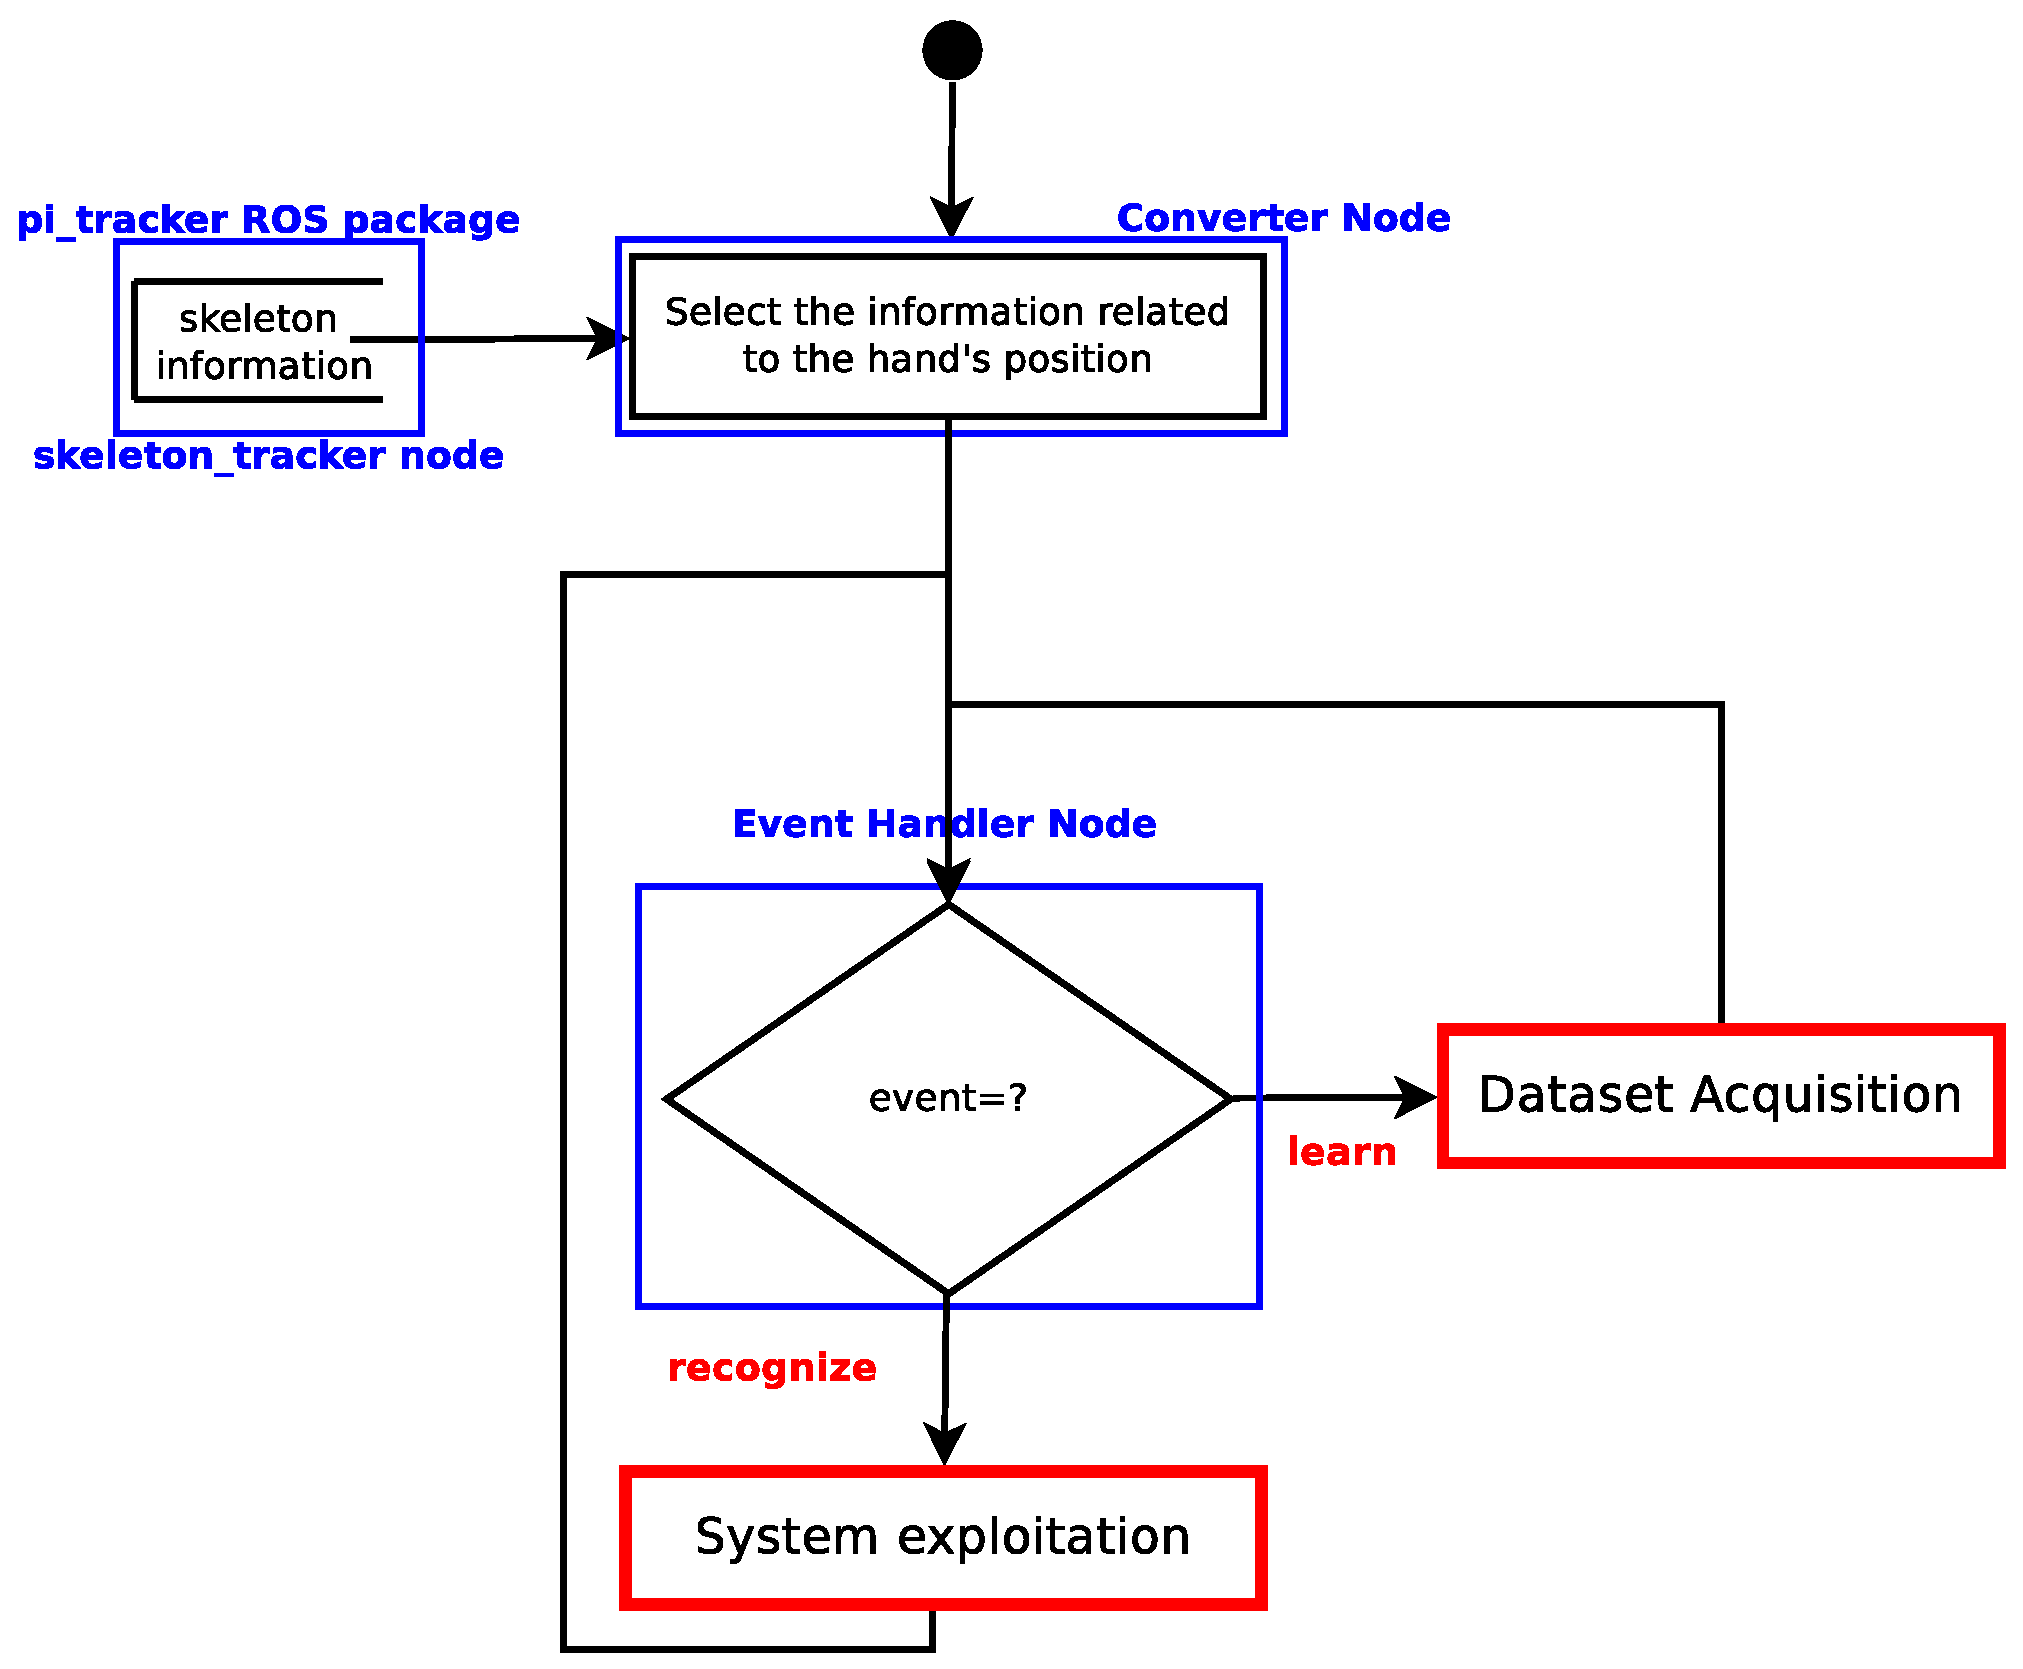
\includegraphics[width=0.8\linewidth]{img/diagrams/flowchart1.eps}
	\caption[General system's flowchart]{General system's flowchart showing the different modes depending on the event}
	\label{flowchart1}
	\end{center}
\end{figure}



% \begin{figure}[H]
% 	\begin{center}
% 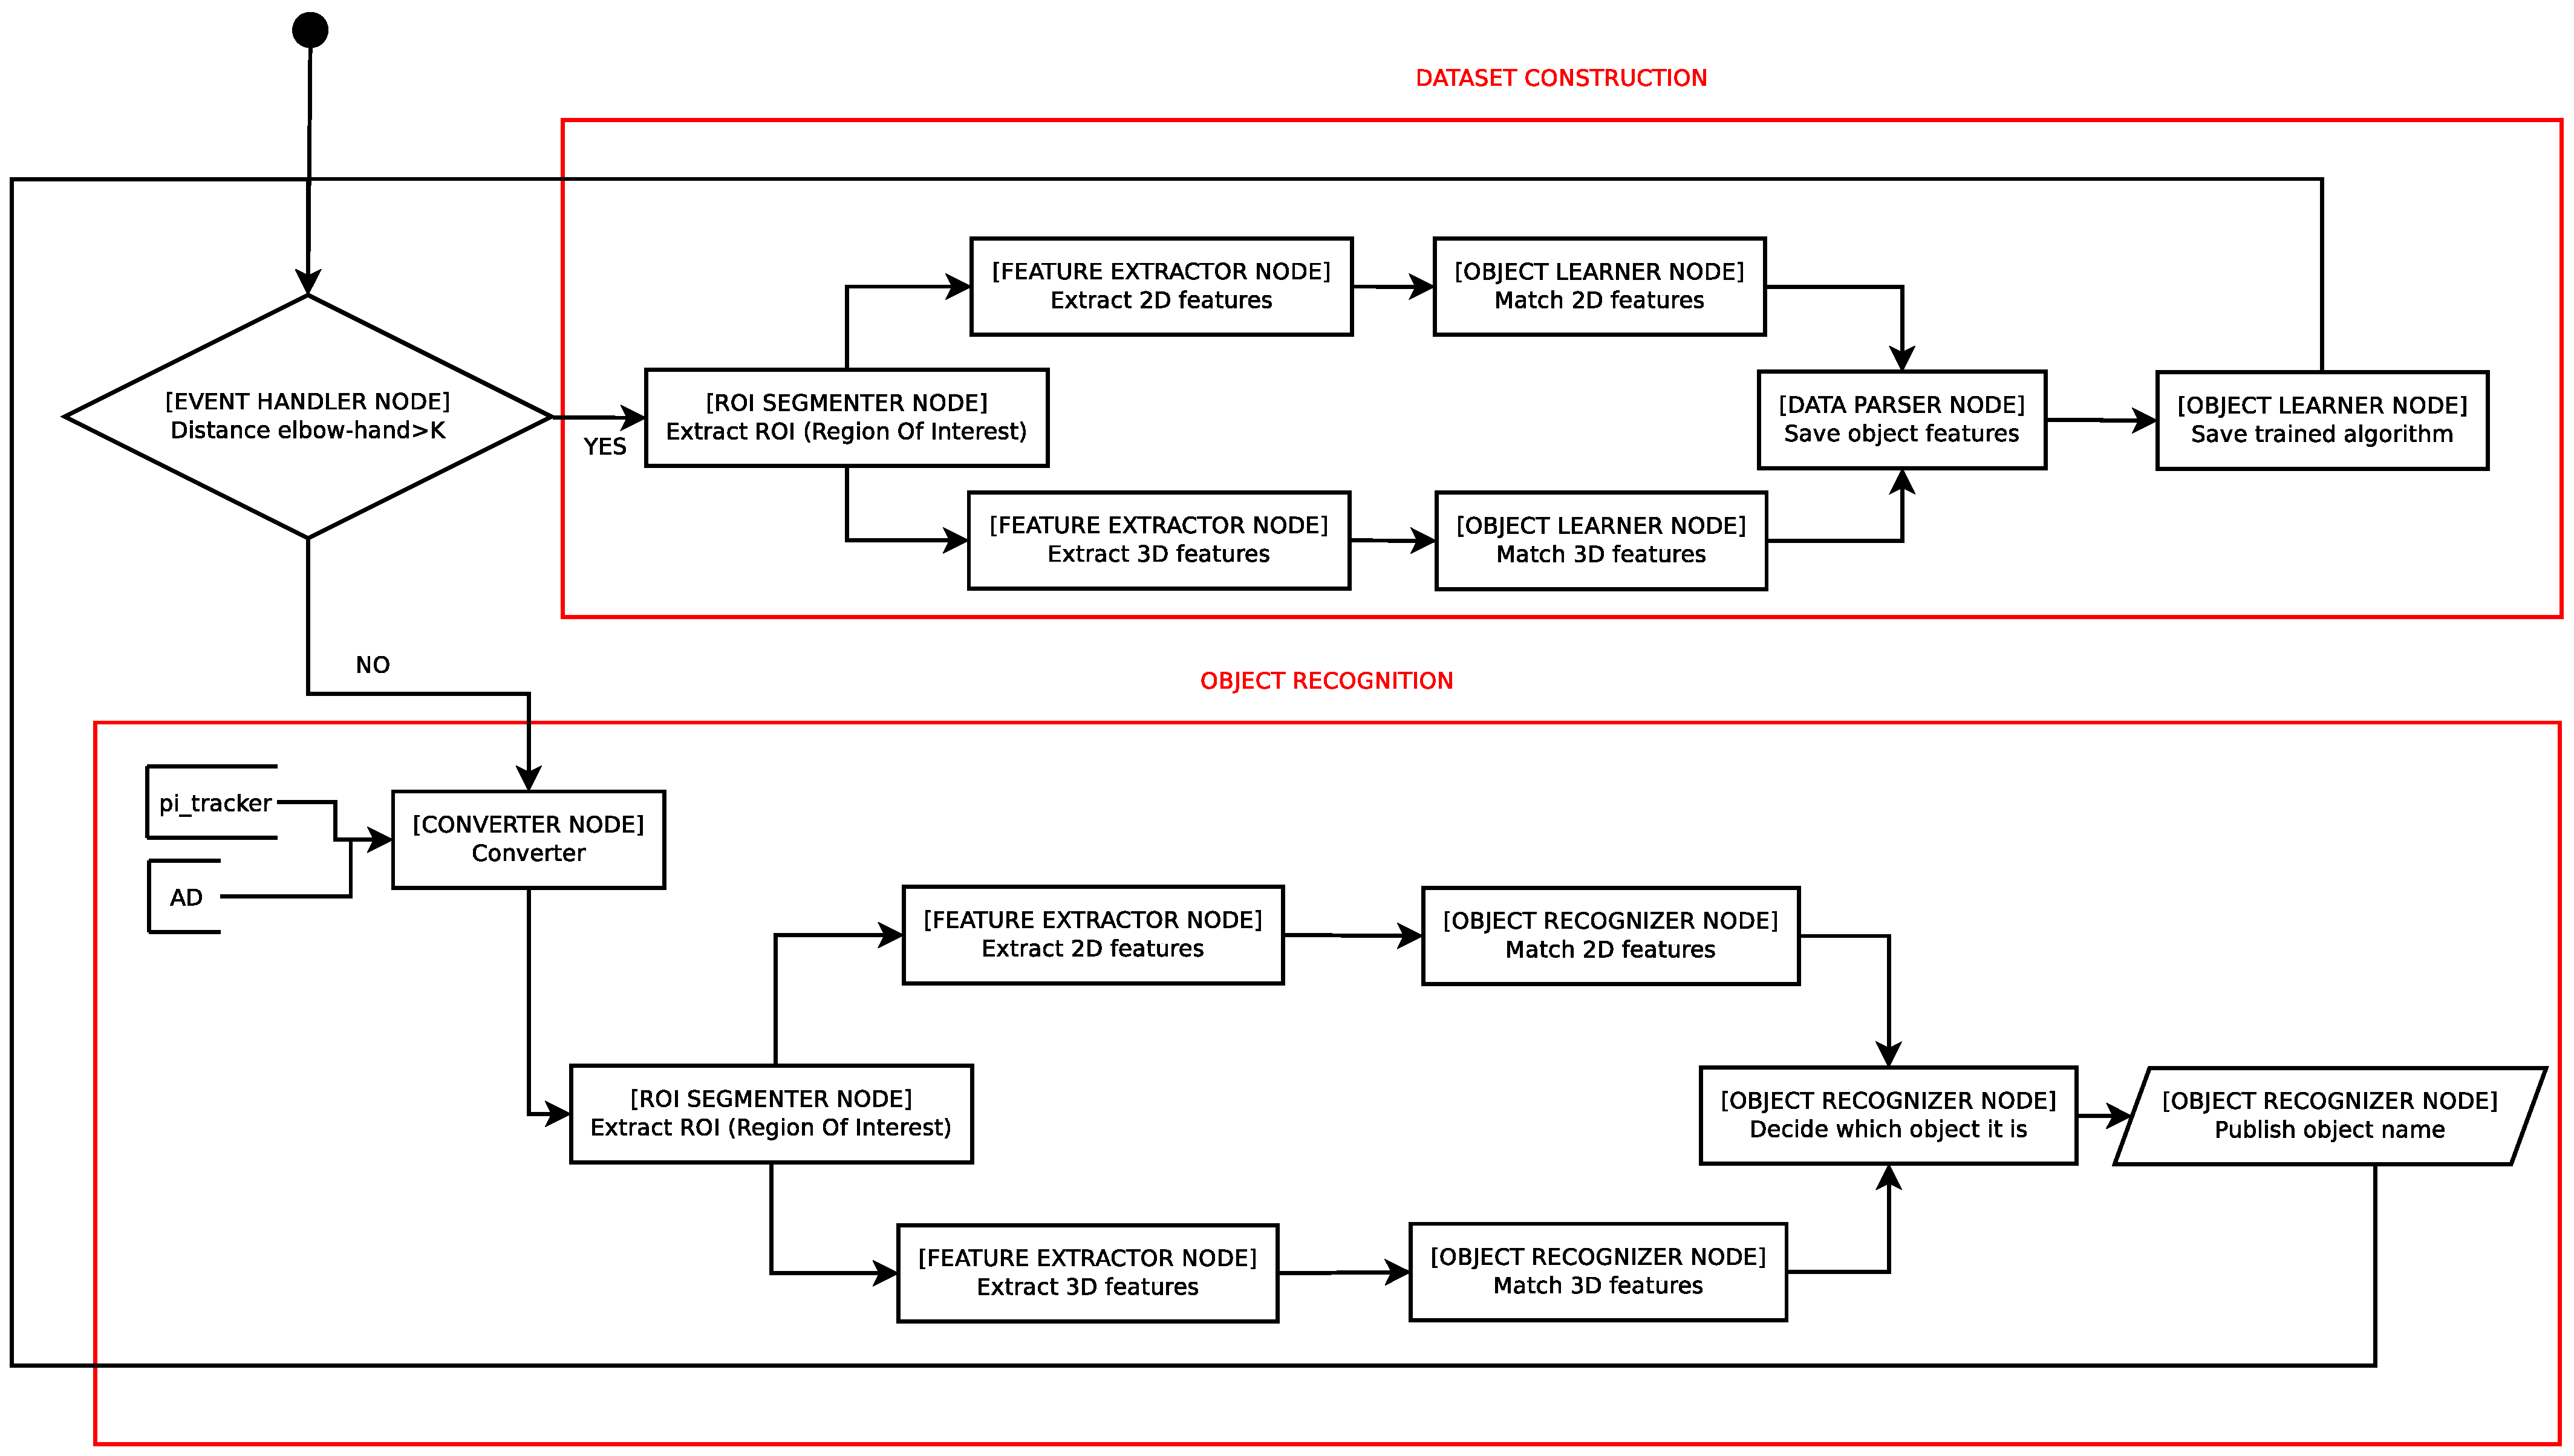
\includegraphics[width=\linewidth]{img/diagrams/flowcharts.eps}
% 	\caption[Software flowchart]{Complete Software flowchart showing the different processing steps between the input and the output}
% 	\end{center}
% 	\label{flowchart}
% \end{figure}

\paragraph{Dataset acquisition or learning mode}\mbox{}
\\

The first step is to extract the ROI (Region of Interest) from the input raw data. 
This is a crucial step that allows to reduce noticeably the amount of time due to computation reducing the size of the processed information. 

Figure \ref{flowchart2} shows the process followed in the segmentation. 
First, the 3D ROI is extracted, and the limits of that region are transformed into pixel coordinates. 
Afterwards, the ROI segmenter 2D node crops the 2D region of interest. 
\begin{figure}[H]
	\begin{center}
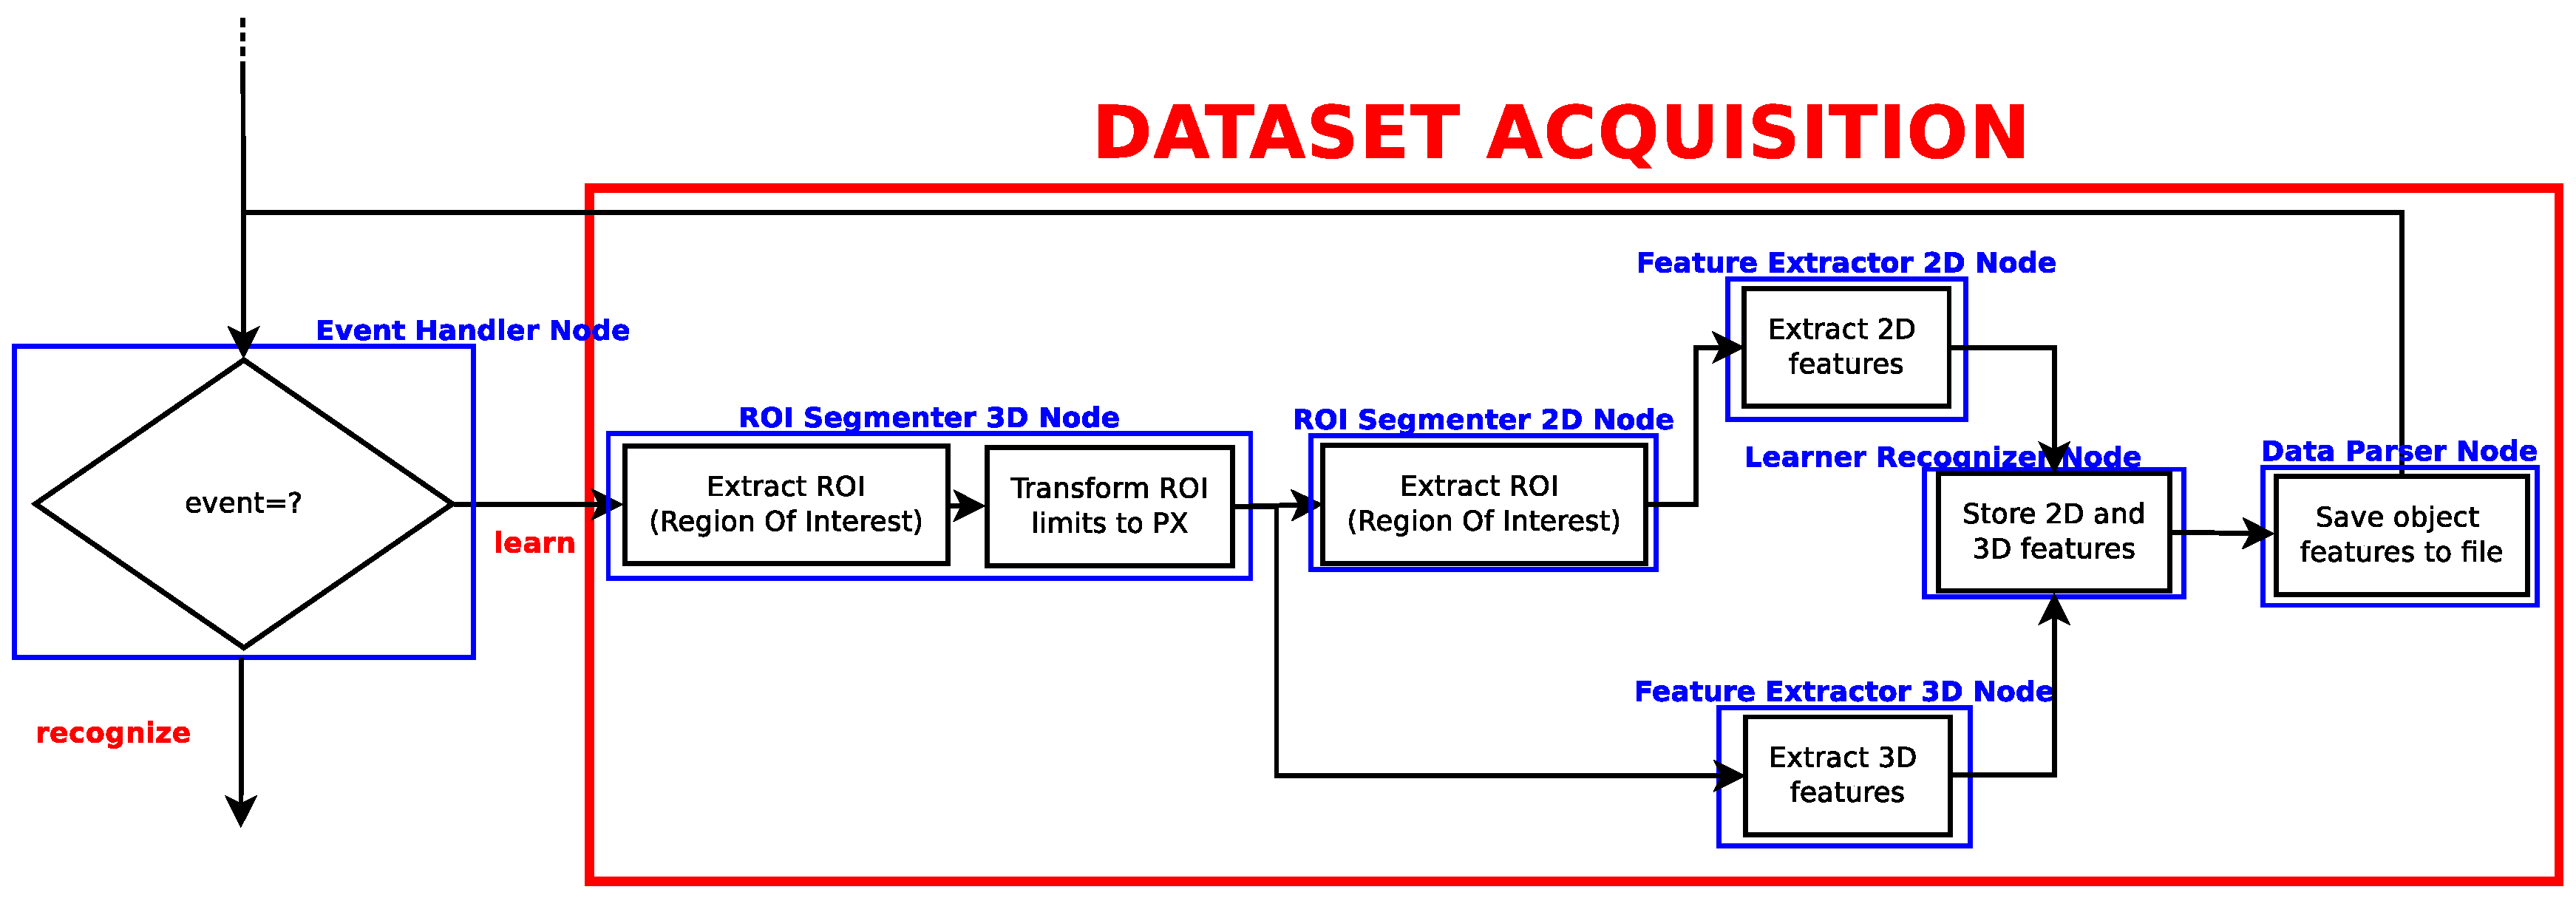
\includegraphics[width=\linewidth]{img/diagrams/flowchart2.eps}
	\caption[Dataset acquisition flowchart]{Flowchart detailing the dataset acquisition or learning mode of the system.}
		\label{flowchart2}

	\end{center}
\end{figure}


\\

After the extraction, the 2D and 3D features of the segmented data are obtained. The features or descriptors are characteristics that define and represent the data from where they were created. 
\\
That is the end of the data cycle of the learning process. 
This cycle is repeated as many times as number of views has been defined in the system. 
As an example, if the software is configured to accept five views per object, the process is repeated five times. 
Between repetitions there is a pause to allow the user to rotate the object and hence obtain as much information as possible. 


\paragraph{System exploitation or recognition mode}\mbox{}


The recognition mode is triggered when the hand is located near the user's body. 
Figure \ref{flowchart3} shows the detailed flowchart of the system exploitation. 
\\
The steps that compose this part of the software are the following: 
First, the input information is converted to the custom message used within the code. Afterwards, as in the previous mode, the Region Of Interest is segmented from both 2D and 3D original information. Then, the descriptors are extracted exactly the same way as in the previous mode. 
\\

\begin{figure}[H]
	\begin{center}
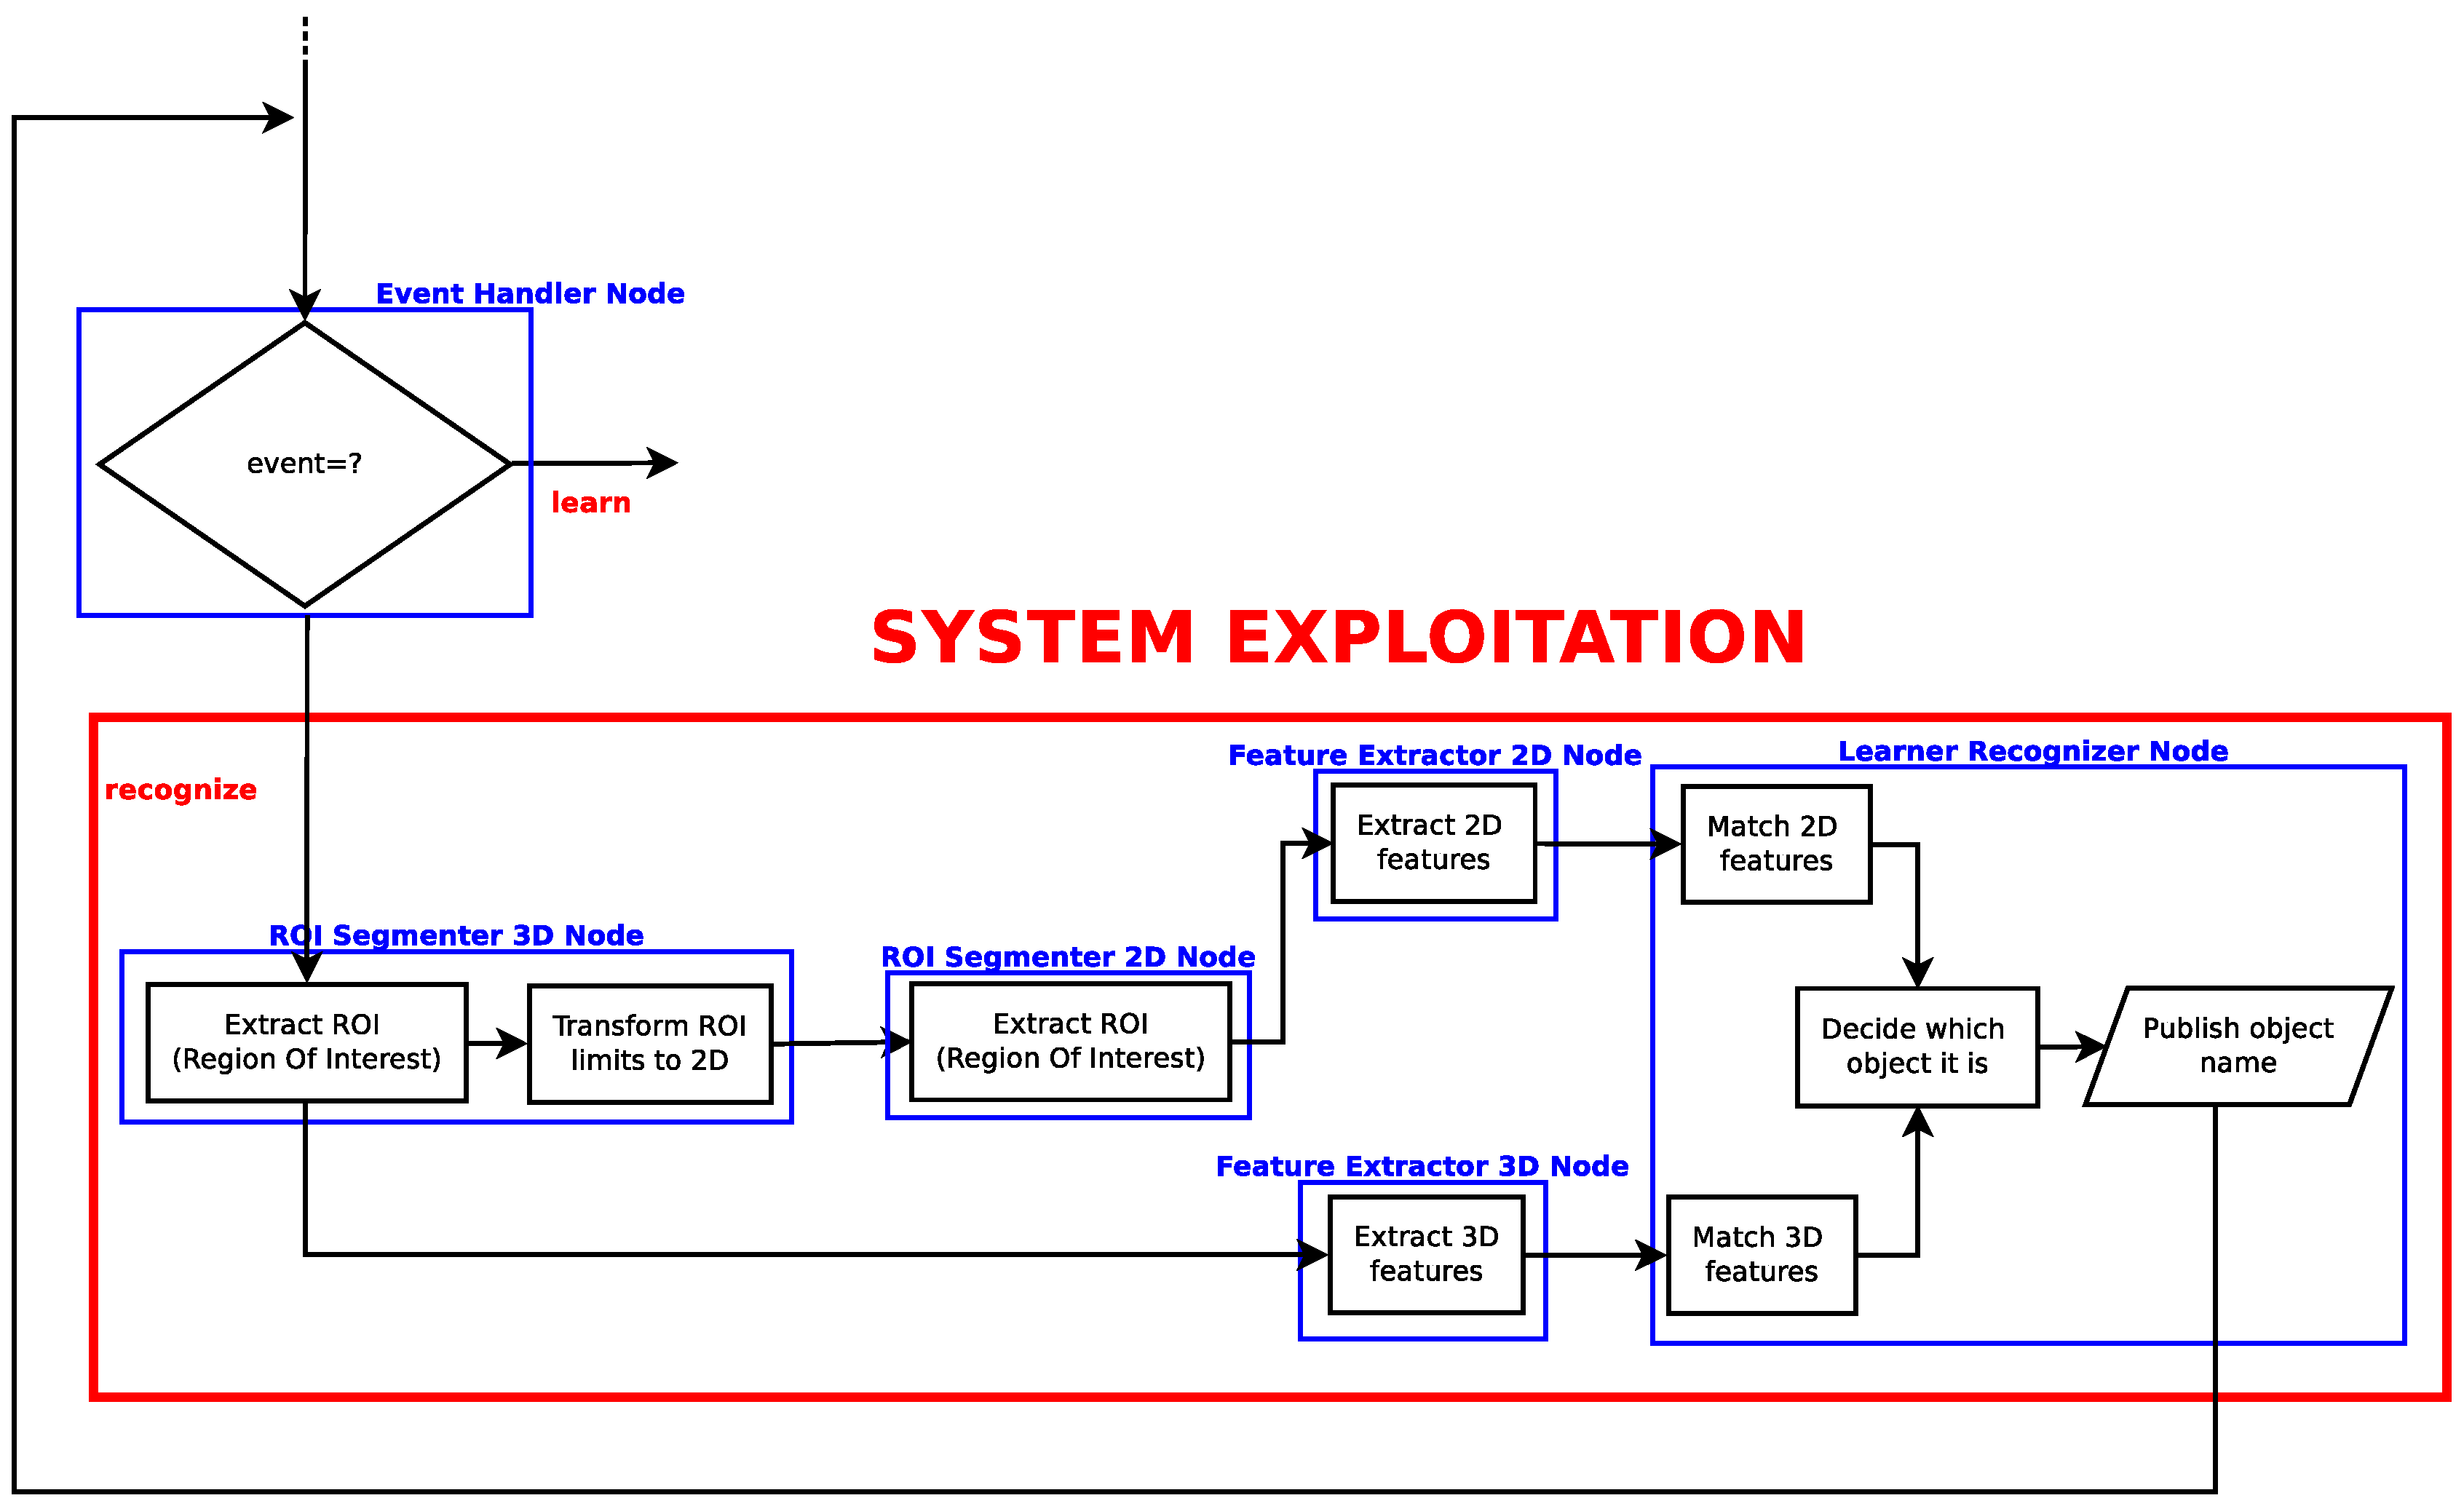
\includegraphics[width=\linewidth]{img/diagrams/flowchart3.eps}
	\caption[System exploitation flowchart]{Flowchart detailing the system exploitation or recognition phase.}
		\label{flowchart3}

	\end{center}
\end{figure}



The next step is the recognition algorithm. This matches the descriptors from both the image and the point cloud and decides which object of the dataset is more similar to the one that is currently on the user's hand. More details about this algorithm may be found in this section. 
\\

Finally, the object identification number is obtained. This data is the output of the system. 
